\documentclass[a4paper,12pt]{article}
\newlength{\outerbordwidth}
\pagestyle{empty}
\pagestyle{plain}
\raggedbottom
\raggedright
\usepackage[svgnames]{xcolor}
\usepackage{framed}
\usepackage{times}
\usepackage{tocloft}
\usepackage{graphicx}
\usepackage{multirow}
\usepackage[utf8]{inputenc}
\usepackage{tabularx}
\title{Omkar-CV}
%-----------------------------------------------------------
%Edit these values as you see fit

\setlength{\outerbordwidth}{0pt}  % Width of border outside of title bars
\definecolor{shadecolor}{gray}{1}  % Outer background color of title bars (0 = black, 1 = white)
\definecolor{shadecolorB}{gray}{0.8}  % Inner background color of title bars


%-----------------------------------------------------------
%Margin setup

\setlength{\evensidemargin}{-0.25in}
\setlength{\headheight}{0in}
\setlength{\headsep}{0in}
\setlength{\oddsidemargin}{-0.25in}
\setlength{\paperheight}{11in}
\setlength{\paperwidth}{8.5in}
\setlength{\tabcolsep}{0in}
\setlength{\textheight}{9.5in}
\setlength{\textwidth}{7in}
\setlength{\topmargin}{-0.3in}
\setlength{\topskip}{0in}
\setlength{\voffset}{0.1in}

\newcommand{\resitem}[1]{\item #1 \vspace{-2pt}}
\newcommand{\resheading}[1]{\vspace{8pt}
    \parbox{\textwidth}{\setlength{\FrameSep}{\outerbordwidth}
        \begin{shaded}
            \setlength{\fboxsep}{0pt}\framebox[\textwidth][l]{\setlength{\fboxsep}{4pt}\fcolorbox{shadecolorB}{shadecolorB}{\textbf{\sffamily{\mbox{~}\makebox[6.762in][l]{\large #1} \vphantom{p\^{E}}}}}}
        \end{shaded}
    }\vspace{-5pt}
}
\newcommand{\ressubheading}[4]{

    \begin{tabular*}{6.5in}{l@{\cftdotfill{\cftsecdotsep}\extracolsep{\fill}}r}
        \textbf{#1} & #2 \\
        \textit{#3} & \textit{#4} \\
    \end{tabular*}\vspace{-6pt}}
%-----------------------------------------------------------


\begin{document}
    
    %-----------------------------------------------------------
    %Insert profile photo 
    \begin{tabular*}{7in}{l@{\extracolsep{\fill}}r}
        & \multirow{1}{*}{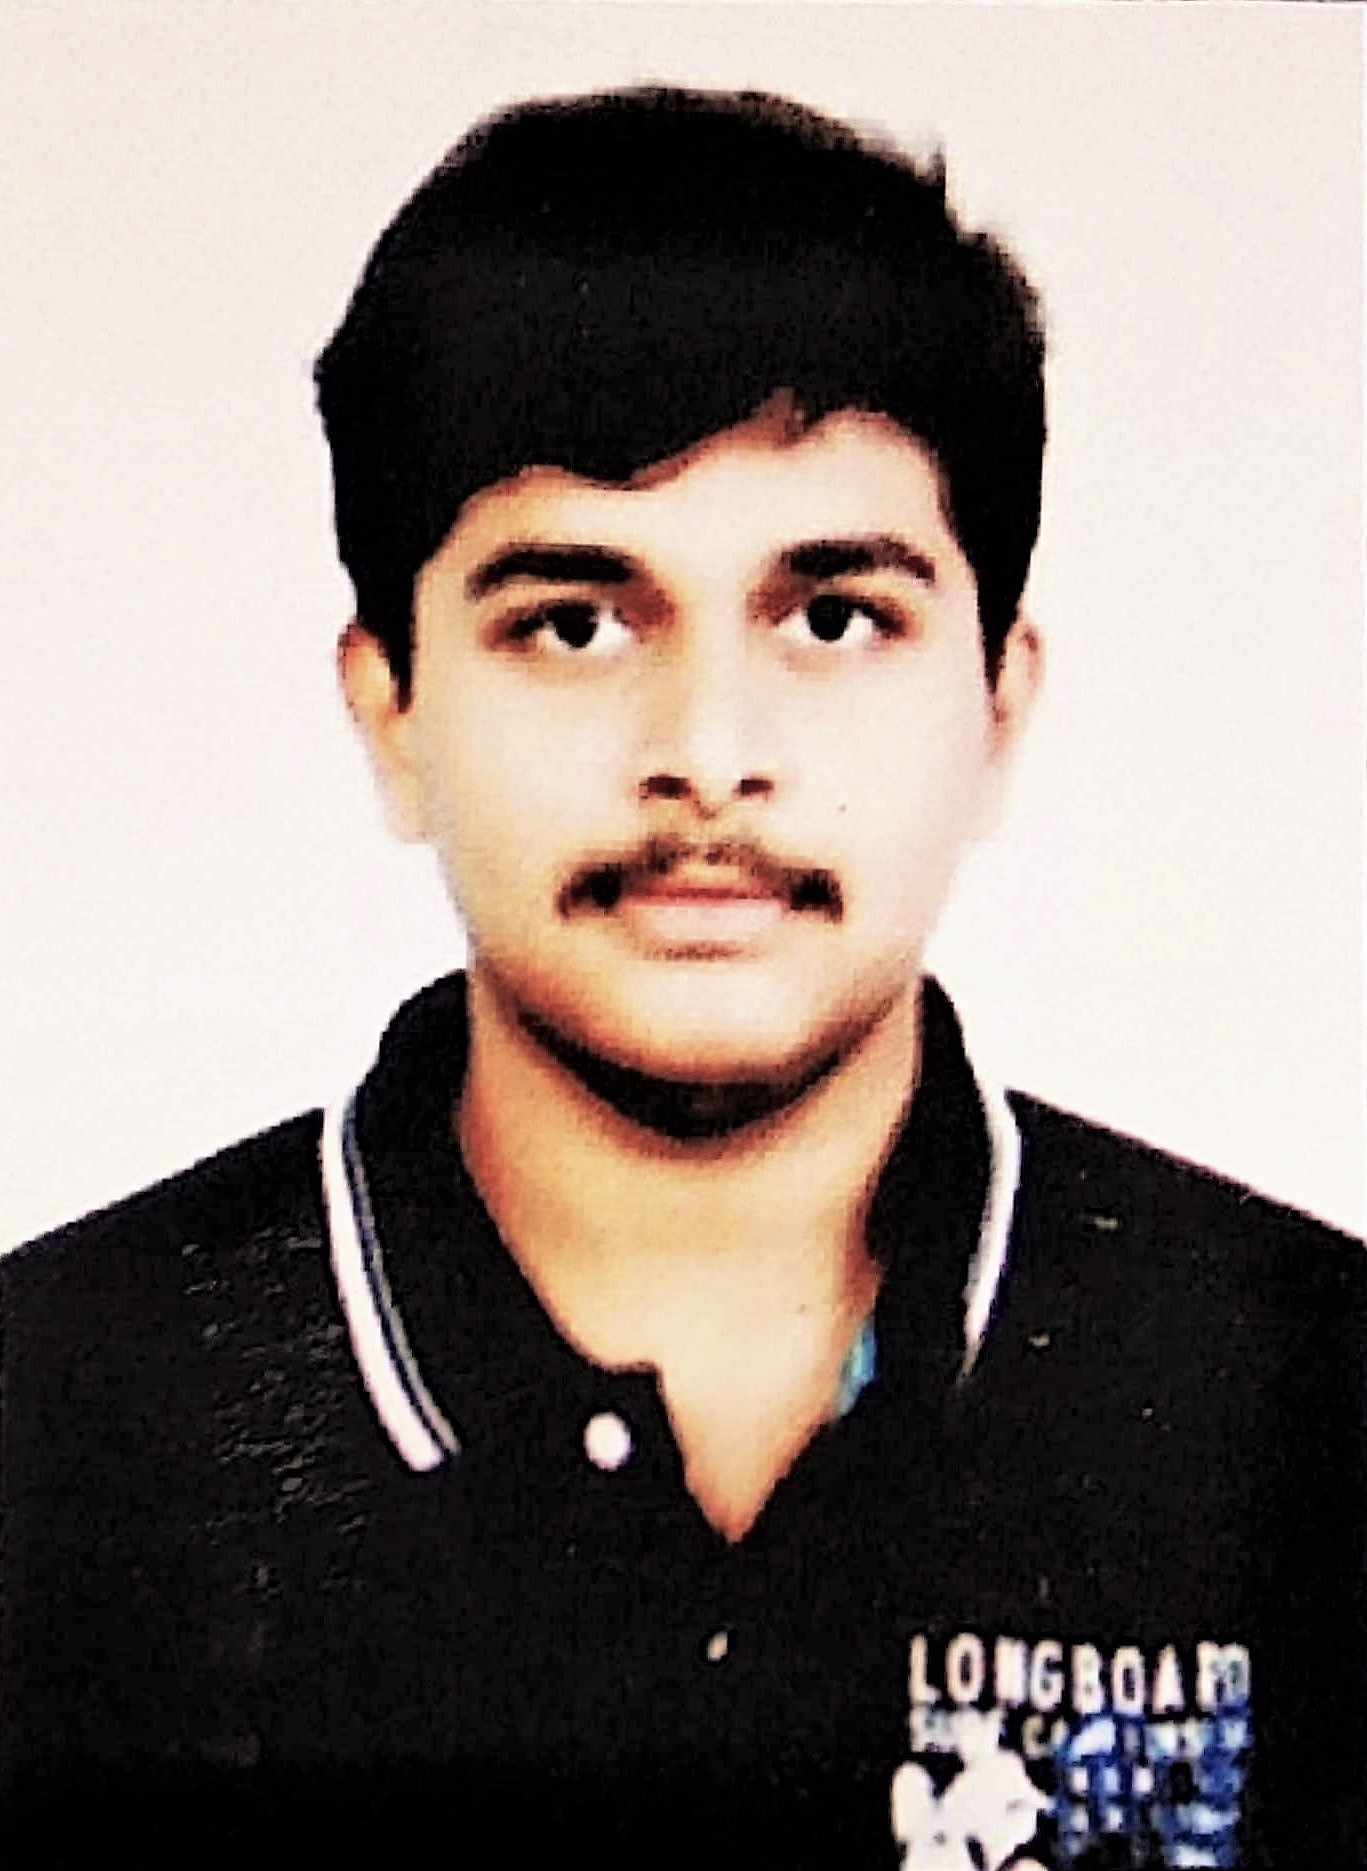
\includegraphics[scale=0.08]{Profile}}\\
         \\
        %-----------------------------------------------------------  
        \textbf{\Large Omkar K. Joshi  } & \\
        Engineering Student & \\
        Fr. Conceicao Rodrigues College of Engineering, Bandra  \\
        omkarjoshi4031@live.com \\
        8007118016\\
    \end{tabular*}
    \\
    %%%%%%%%%%%%%%%%%%%%%%%%%%%%%%
    \resheading{Objective}
    %%%%%%%%%%%%%%%%%%%%%%%%%%%%%%
    \begin{itemize}
        \item
            I am seeking a competitive and challenging environment where I can serve your organization and establish a career for myself.
    \end{itemize}
    %%%%%%%%%%%%%%%%%%%%%%%%%%%%
    \resheading{Education}
    %%%%%%%%%%%%%%%%%%%%%%%%%%%%%%
    \begin{itemize}
        \item
        \ressubheading{Fr. Conceicao Rodrigues College of Engineering}{Mumbai University}{B. Engineering Electronics}{Pursuing}
        \begin{itemize}
            \resitem{Second Year: 7.035 CGPA}
            \resitem{Third Year: Pursuing }
        \end{itemize}
        
        \item
        \ressubheading{Viva College of Diploma Engineering And Technology}{MSBTE}{Diploma in Electronics and Telecommunication}{2016}
        \begin{itemize}
            \resitem{Graduated with a 82\% average}
        \end{itemize}
    
        \item
        \ressubheading{St. Augustine's High School}{Mumbai Board}{High School}{2013}
        \begin{itemize}
            \resitem{Graduated with a 81\% average}
        \end{itemize}
    \end{itemize}
    %%%%%%%%%%%%%%%%%%%%%%%%%%%%%%
    \resheading{Projects}
    %%%%%%%%%%%%%%%%%%%%%%%%%%%%%%
    \begin{itemize}
        \item
        \ressubheading{Gesture Vocalizer for deaf People}{}{Diploma Final Year Project.}{}
        \begin{itemize}
            \resitem{Involved flex sensor for gesture recognition.}
        \end{itemize}
        
        \item 
        \ressubheading{Autonomus Car Using CNN }{}{Degree Third Year.}{}
        \begin{itemize}
            \resitem{An AI was trainned for driving a RC car.}
            \resitem{It had dataset around 12,000 labled images, obtained from udacity open source car simulator.}
            \resitem{Written on Keras.}
        \end{itemize}
        
        \item
        \ressubheading{Automatic Traffic Surveillance System}{}{Degree Third Year.}{}
        \begin{itemize}
            \resitem{Group project, worked on character recognition using CNN and speed detection using openCV.}
            \resitem{Highly modified CAR-74 dataset. It contained 115,200 labled images.}
            \resitem{Written on Tflearn.}
        \end{itemize}
    
        \item
        \ressubheading{Natural Language Processing}{}{Degree Third Year.}{}
        \begin{itemize}
            \resitem{It is an ongoing project. Here an AI is designed to understands simple speech commands.}
            \resitem{Kaggle dataset is used.}
            \resitem{Writing on Tflearn.}
        \end{itemize}
    \end{itemize}

    %%%%%%%%%%%%%%%%%%%%%%%%%%%%%%
    \resheading{Training}
    %%%%%%%%%%%%%%%%%%%%%%%%%%%%%%
    \begin{itemize}
        \resitem{Machine learning from}\textit{"Coursera"} {Andrew Ng.}
        \resitem{Python from}\textit{"TheNewBoston"}{an youtube channel.}
        \resitem{OpenCV from}\textit{"Sentdex"}{an youtube channel.}
    \end{itemize}
    
     %%%%%%%%%%%%%%%%%%%%%%%%%%%%%%
    \resheading{Technical Skills}
     %%%%%%%%%%%%%%%%%%%%%%%%%%%%%%
    \begin{itemize}
        \resitem{{\bf Programing Languages:} Python, OpenCv, Html, Java, C++, MySql}
        \resitem{{\bf Software:} \LaTeX, Adobe Photoshop, Adobe Illustrator, Adobe After Effects, Matlab, Cinema 4D, FL-studio, Zbrush, V-Rev, LT-spice, Autocad.}
    \end{itemize}

     %%%%%%%%%%%%%%%%%%%%%%%%%%%%%%
    \resheading{Soft Skills}
    %%%%%%%%%%%%%%%%%%%%%%%%%%%%%%
    \begin{itemize}
        \resitem{Self-Motivation and Responsibility}
        \resitem{Leadership and Teamwork}
        \resitem{Ability to Work Under Pressure and Time Management}
        \resitem{Negotiation and Conflict Resolution}
        
    \end{itemize}
 
     %%%%%%%%%%%%%%%%%%%%%%%%%%%%%%
    \resheading{Achievements}
    %%%%%%%%%%%%%%%%%%%%%%%%%%%%%%
    \begin{itemize}
       \resitem{Entitled with \textit{"Best Algorithm"} at E-yantra National Project Competition, IIT Bombay}\\
       \resitem{Passed elementary and intermediate drawing exam}\\
    \end{itemize}
    
     %%%%%%%%%%%%%%%%%%%%%%%%%%%%%%
    \resheading{Co-curricular Activity}
    %%%%%%%%%%%%%%%%%%%%%%%%%%%%%%
    \begin{itemize}
        \resitem{IEEE-CRCE \textit{"Design Head"}.}
        \resitem{Appointed as \textit{"Training Placement Coordinator"}of Fr.CRCE}
        \resitem{Participated in National Level Project Competition.}
        \resitem{Participated in State Level Hackthon.}
    \end{itemize}
    %%%%%%%%%%%%%%%%%%%%%%%%%%%%%%
    \resheading{Personal Details}
    %%%%%%%%%%%%%%%%%%%%%%%%%%%%%%
    \begin{itemize}
        \resitem{{\bf Father's Name:} Kirtinandan J Joshi}
        \resitem{{\bf Mother's Name:} Nandini K Joshi}
        \resitem{{\bf Sex:} Male}
        \resitem{{\bf Date of Birth:} 2\textsuperscript{nd} July 1997}
        \resitem{{\bf Nationality:} Indian}
        \resitem{{\bf Marital Status:} Single}
        \resitem{{\bf Hobbies:} Reading Sci-Fic books, Listening Music, Video gaming, Cooking.}
    \end{itemize}


    %%%%%%%%%%%%%%%%%%%%%%%%%%%%%%
    \resheading{Declaration}
    %%%%%%%%%%%%%%%%%%%%%%%%%%%%%%
    \begin{itemize}
        \item
        All the information mentioned in the resume are correct to the best of my knowledge and believe.\\
    \end{itemize}
    
    
    \begin{flushright}
        \small -April 18, 2018
    \end{flushright}
    
\end{document}